\documentclass[12pt]{llncs}

\usepackage[utf8]{inputenc}
\usepackage[T1]{fontenc}
\usepackage{amsmath}
\usepackage{amssymb}
\usepackage{mathtools}
\usepackage{parskip}
\usepackage{tikz}
\usepackage{subcaption}

\usetikzlibrary{arrows}

\captionsetup{compatibility=false}

\DeclarePairedDelimiter{\set}{\{}{\}}
\DeclarePairedDelimiter{\tuple}{(}{)}
\DeclarePairedDelimiter{\abs}{\lvert}{\rvert}

\let\oldleq\leq
\renewcommand{\leq}[1][]{\oldleq_{#1}}
\renewcommand{\implies}{\rightarrow}

\newcommand{\comment}[1]{\texttt{COMMENT TO BOW YAW:\\#1}}
\newcommand{\bye}[1]{}
\newcommand{\bicond}{\leftrightarrow}
\newcommand{\poset}[1]{\mathcal{#1}}
\newcommand{\uni}[1][]{\Omega_{#1}}
\newcommand{\lang}[1]{L(#1)}
\newcommand{\lin}[1]{\texttt{#1}}
\newcommand{\swap}[1][]{\leftrightarrow_{#1}}
\newcommand{\sgraph}[1]{G(#1)}
\newcommand{\lext}{\sqsubseteq}
\newcommand{\incomp}{\parallel}
\newcommand{\covered}{\prec}
\newcommand{\complmt}[1]{\overline{#1}}
\newcommand{\satvar}[2]{\mathtt{X}_{#1}^{#2}}
\newcommand{\bigo}[1]{\mathcal{O}(#1)}

\begin{document}

\title{Poset Paper}
\author{Bow-yaw Wang\inst{1} \and Chih-chen Yuan\inst{2}}
\institute{Academia Sinica, Taiwan\\ \and
National Taiwan Normal University, Taiwan}
\maketitle

\begin{abstract}
hello world
\end{abstract}

\section{Introduction}
Intro part here
% intro pcp
% intro converse of lin
% intro trivial case by Szpilrajn corollary
% intro trivial non-max solution?
% intro np completeness?

\section{Preliminaries}
A \emph{partial order} is a binary relation that is reflexive, antisymmetric, and transitive. A \emph{partially ordered set} or \emph{poset} is a binary structure $\poset{P} = \tuple{\uni, \leq}$ where the \emph{universe} $\uni$ is a set and $\leq$ is a partial order on $\uni$; we refer to members of $\uni$ as elements of $\poset{P}$ and, where specificity is desired, to $\uni$ as $\uni[
\poset{P}]$ and $\leq$ as $\leq[\poset{P}]$.

% example:posetp
\begin{example}
    For the following definition, consider the poset $\poset{P}$ over $\set{a,b,c,d}$ with $a \leq b$\ ; $a \leq c$\ ; $a \leq d$\ ; $b \leq d$\ ; and $c \leq d$. Figure~\ref{figure:posetp} describes $\poset{P}$ with a graph $\tuple{V,E} = \tuple{\Omega,\covered}$.
    \label{example:posetp}
\end{example}

\vspace{-15px}
% figure:posetp
\begin{figure}
    \centering
    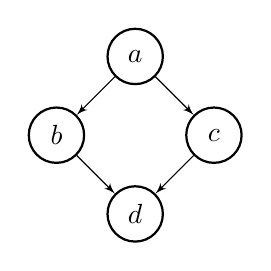
\begin{tikzpicture}
        [
        vertex/.style={circle,thick,draw,minimum size=2em},
        edge/.style={->,> = latex'}
        ]
    \node[vertex] (1) at (1,2) {$a$};
    \node[vertex] (2) at (0,1) {$b$};
    \node[vertex] (3) at (2,1) {$c$};
    \node[vertex] (4) at (1,0) {$d$};
    \draw[edge] (1) -- (2);
    \draw[edge] (1) -- (3);
    \draw[edge] (2) -- (4);
    \draw[edge] (3) -- (4);
    \end{tikzpicture}
    \caption{Graph representation of $\poset{P}$ from Example~\ref{example:posetp}.}
    \label{figure:posetp}
\end{figure}
\vspace{-15px}

The \emph{cover} relation $\covered$ of a poset $\poset{P}$ is the transitive reduction of its order relation; it describes the case of immediate successor: for $x, y \!\in\! \poset{P}$, $x \covered y$ if and only if $x \leq y$ and there is no $z \!\in\! \poset{P}$ such that $x \lneq z$ and $z \lneq y$. For Example~\ref{example:posetp}, the covered relation includes $a \covered b$\ ; $a \covered c$\ ; $b \covered d$\ ; and $c \covered d$. Note that $\tuple{a,d}$ is absent in $\covered$.

In addition, we describe the case of \emph{incomparability} in a poset $\poset{P}$ with $\incomp$ relation: for $x, y \!\in\! \poset{P}$, $x \incomp y$ if and only if $x \nleq y$ and $y \nleq x$. For Example~\ref{example:posetp}, there is $b \incomp c$.

% example:posetl
\begin{example}
    For the following definition, consider the poset $\poset{L}$ over $\set{a,b,c,d}$ with $a \leq b$\ ; $a \leq c$\ ; $a \leq d$\ ; $b \leq c$\ ; $b \leq d$\ ; and $c \leq d$. Figure~\ref{figure:posetl} represents $\poset{L}$ with a graph $\tuple{V,E} = \tuple{\uni,\covered}$.
    \label{example:posetl}
\end{example}

\vspace{-15px}
% figure:posetl
\begin{figure}
    \centering
    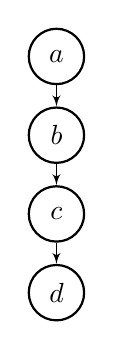
\begin{tikzpicture}
        [
        vertex/.style={circle,thick,draw,minimum size=2em},
        edge/.style={->,> = latex'}
        ]
    \node[vertex] (1) at (0,3) {$a$};
    \node[vertex] (2) at (0,2) {$b$};
    \node[vertex] (3) at (0,1) {$c$};
    \node[vertex] (4) at (0,0) {$d$};
    \draw[edge] (1) -- (2);
    \draw[edge] (2) -- (3);
    \draw[edge] (3) -- (4);
    \end{tikzpicture}
    \caption{Graph representation of $\poset{L}$ from Example~\ref{example:posetl}.}
    \label{figure:posetl}
\end{figure}
\vspace{-15px}

A partial order where every pair of elements is comparable is called a \emph{linear order}, and a poset $\poset{L}$ with such an order is called a \emph{linear poset}; that is, for $x, y \!\in\! \poset{L}$, $x \leq y$ or $y \leq x$. Note that the graph describing a linear poset is a path. For simplicity, we represent a linear poset in string form. For Example~\ref{example:posetl}, we write \lin{abcd}.

A linear poset $\poset{L}$ that extends a poset $\poset{P}$ is called a \emph{linear extension} or \emph{linearization} of $\poset{P}$, denoted $\poset{P} \lext \poset{L}$; that is, for posets $\poset{P},\poset{L}$ with $\uni[P] \!=\! \uni[L]$, $\poset{P} \lext \poset{L}$ if and only if $\poset{L}$ is linear and $\leq[P] \>\subseteq\> \leq[L]$. For example, for $\poset{P}$ from Example~\ref{example:posetp} and $\poset{L}$ from Example~\ref{example:posetl}, $\poset{P} \lext \poset{L}$. Note that a linearization of a poset is equivalent to a topological sort of the graph describing that poset.

Every poset admits a set of linearizations. The set of all linearizations of a poset $\poset{P}$ is denoted $\lang{\poset{P}}$. We shall consider it the \emph{language} of $\poset{P}$. For $\poset{P}$ from Example~\ref{example:posetp}, we have $\lang{\poset{P}} = \set{\lin{abcd},\lin{acbd}}$. For $\poset{L}$ from Example~\ref{example:posetl}, $\lang{\poset{L}} = \set{\lin{abcd}}$.

Now, we are ready to define \emph{Poset Cover Problem}.

% definition:pcp
\begin{definition}[Poset Cover Problem]
    Given a set of linear posets $\Upsilon$, find a set of partial orders $C$, called a cover, such that $\abs{C}$ is minimal and the union of the languages of posets in $C$ is equal to $\Upsilon$; that is, $\Upsilon = \bigcup_{\poset{P} \in C} \lang{\poset{P}}$.
    \label{definition:pcp}
\end{definition}

% example:cover example
\begin{example}
    Given the set of linear posets $\set{\lin{abfce},\lin{bafce},\lin{abcfe},\lin{abfec}}$ over $\set{a,b,c,f,e}$, a minimal poset cover of two posets $\poset{A},\poset{B}$ is shown in Figure~\ref{figure:cover example c} with ${\lang{\poset{A}} = \set{\lin{abfce},\lin{abcfe},\lin{abfec}}}$ and ${\lang{\poset{B}} = \set{\lin{bafce}}}$.
    \label{example:cover example}
\end{example}

\vspace{-15px}
% figure:cover example
\begin{figure}
    % figure:cover example c
    \begin{subfigure}[b]{0.5\textwidth}
        \centering
        \begin{subfigure}[b]{0.4\textwidth}
            \centering
            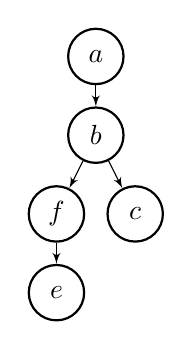
\begin{tikzpicture}
                [
                vertex/.style={circle,thick,draw,minimum size=2em},
                edge/.style={->,> = latex'}
                ]
            \node[vertex] (1) at (1,4) {$a$};
            \node[vertex] (2) at (1,3) {$b$};
            \node[vertex] (3) at (0.5,2) {$f$};
            \node[vertex] (4) at (0.5,1) {$e$};
            \node[vertex] (5) at (1.5,2) {$c$};
            \draw[edge] (1) -- (2);
            \draw[edge] (2) -- (3);
            \draw[edge] (3) -- (4);
            \draw[edge] (2) -- (5);
            \end{tikzpicture}
            \caption*{Poset $\poset{A}$}
        \end{subfigure}%
        \begin{subfigure}[b]{0.4\textwidth}
            \centering
            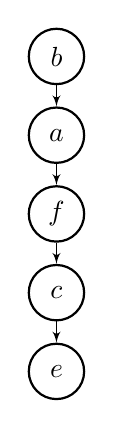
\begin{tikzpicture}
                [
                vertex/.style={circle,thick,draw,minimum size=2em},
                edge/.style={->,> = latex'}
                ]
            \node[vertex] (6) at (4,4) {$b$};
            \node[vertex] (7) at (4,3) {$a$};
            \node[vertex] (8) at (4,2) {$f$};
            \node[vertex] (9) at (4,1) {$c$};
            \node[vertex] (10) at (4,0) {$e$};
            \draw[edge] (6) -- (7);
            \draw[edge] (7) -- (8);
            \draw[edge] (8) -- (9);
            \draw[edge] (9) -- (10);
            \end{tikzpicture}
            \caption*{Poset $\poset{B}$}
        \end{subfigure}
        \caption{A minimal cover.}
        \label{figure:cover example c}
    \end{subfigure}%
    % figure:cover example c'
    \begin{subfigure}[b]{0.5\textwidth}
        \centering
        \begin{subfigure}[b]{0.4\textwidth}
            \centering
            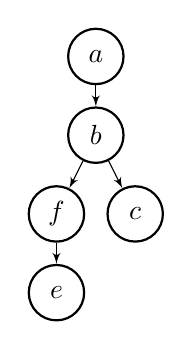
\begin{tikzpicture}
                [
                vertex/.style={circle,thick,draw,minimum size=2em},
                edge/.style={->,> = latex'}
                ]
            \node[vertex] (1) at (1,4) {$a$};
            \node[vertex] (2) at (1,3) {$b$};
            \node[vertex] (3) at (0.5,2) {$f$};
            \node[vertex] (4) at (0.5,1) {$e$};
            \node[vertex] (5) at (1.5,2) {$c$};
            \draw[edge] (1) -- (2);
            \draw[edge] (2) -- (3);
            \draw[edge] (3) -- (4);
            \draw[edge] (2) -- (5);
            \end{tikzpicture}
            \caption*{Poset $\poset{C}$}
        \end{subfigure}%
        \begin{subfigure}[b]{0.4\textwidth}
            \centering
            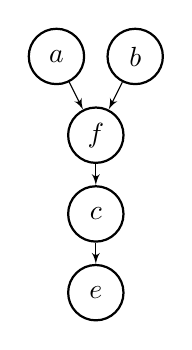
\begin{tikzpicture}
                [
                vertex/.style={circle,thick,draw,minimum size=2em},
                edge/.style={->,> = latex'}
                ]
            \node[vertex] (6) at (3.5,4) {$a$};
            \node[vertex] (7) at (4.5,4) {$b$};
            \node[vertex] (8) at (4,3) {$f$};
            \node[vertex] (9) at (4,2) {$c$};
            \node[vertex] (10) at (4,1) {$e$};
            \draw[edge] (6) -- (8);
            \draw[edge] (7) -- (8);
            \draw[edge] (8) -- (9);
            \draw[edge] (9) -- (10);
            \end{tikzpicture}
            \caption*{Poset $\poset{D}$}
        \end{subfigure}
        \caption{Another minimal cover.}
        \label{figure:cover example c'}
    \end{subfigure}
    \caption{Minimal covers for the set $\set{\lin{abfce},\lin{bafce},\lin{abcfe},\lin{abfec}}$.}
    \label{figure:cover example}
\end{figure}
\vspace{-15px}

A minimal poset cover may not be unique, and the languages of the posets in a cover may overlap. For Example~\ref{example:cover example}, there is another minimal poset cover, shown in Figure~\ref{figure:cover example c'}, with overlapping languages ${\lang{\poset{C}} = \set{\lin{abfce},\lin{abcfe},\lin{abfec}}}$ and ${\lang{\poset{D}} = \set{\lin{abfce},\lin{bafce}}}$.

\section{Reduction to SAT}
Since the poset cover problem is proved to be NP-complete, we  reduce the problem to SAT to utilize the power of modern SAT solvers. However, a naive encoding would easily result in superpolynomial transformation. We shall first show where the naive encoding falls short and then present a more efficient method.

\subsection{Basic Constraints}
Before getting into constraints given by the problem, here we give the definitions and constraints for the basic poset construction.

\subsubsection{Variable Semantics}
For a poset $\poset{P}$ and $x \!\neq\! y \!\in\! \uni$, we encode with the propositional variable $\satvar{x,y}{\poset{P}}$ the case that $x \leq[\poset{P}] y$.

\subsubsection{Poset Axioms}
Only antisymmetry and transitivity are relevant in our reduction. For a poset $\poset{P}$, we enforce antisymmetry with
\[
\bigwedge_{x \neq y \in \uni} \neg (\satvar{x,y}{\poset{P}} \wedge \satvar{y,x}{\poset{P}})
\]
and transitivity with
\[
\bigwedge_{x \neq y \neq z \in \uni}
\satvar{x,y}{\poset{P}} \wedge \satvar{y,z}{\poset{P}} \implies \satvar{x,z}{\poset{P}}
\]

\subsubsection{Linearization Constraints}
For posets $\poset{P},\poset{L}$ with $\poset{P} \lext \poset{L}$, we encode axioms for both $\poset{P}$ and $\poset{L}$ and add per definition
\[
\bigwedge_{x \neq y \in \uni} \satvar{x,y}{\poset{P}} \implies \satvar{x,y}{\poset{L}}
\]
Within logical formulae, we shall abuse the notation $\poset{P} \lext \poset{L}$ as a macro for the above formula.

\comment{I'm not sure if this is okay but it can reduce one quantifier in later formulae}

\subsection{Problem Constraints}
Our goal is to find a minimal set $C$ of posets such that $\bigcup_{\poset{P} \in C} \lang{\poset{P}}$ is equal to the input set of linear posets $\Upsilon$. To ensure we find the minimal cover, we encode the case when $\abs{C} = k$, starting from $k = 1$, and incrementally query SAT solver.

\begin{enumerate}
    \item Let $k = 1$.
    \item Encode the case and query solver.
    \item If a solution is found, we are done. Else, let $k = k+1$ and go to step 2.
\end{enumerate}

The poset cover problem can now be restated in logical formulae. Given $\Upsilon$ and the size of the cover $k$, we first construct $k$ posets by encoding their axioms. Next, we encode axioms for all the posets in $\Upsilon$ and then specify their order relations accordingly.

We shall encode the problem constraints, $\Upsilon = \bigcup_{\poset{P} \in C} \lang{\poset{P}}$, in a twofold manner, by separately constraining $\Upsilon \subseteq \bigcup_{\poset{P} \in C} \lang{\poset{P}}$ and $\Upsilon \supseteq \bigcup_{\poset{P} \in C} \lang{\poset{P}}$.

\subsubsection{Naive Method} A straightforward way to encode the problem follows immediately from the definition.

For $\Upsilon \subseteq \bigcup_{\poset{P} \in C} \lang{\poset{P}}$, it effectively states that every $\poset{L} \!\in\! \Upsilon$ is a linearization of some $\poset{P} \!\in\! C$. We encode it as
\[
\bigwedge_{\poset{L} \in \Upsilon} \bigvee_{\poset{P} \in C} \poset{P} \lext \poset{L}
\]

For $\Upsilon \supseteq \bigcup_{\poset{P} \in C} \lang{\poset{P}}$, conversely, it states that every $\poset{L} \!\not\in\! \Upsilon$ is not a linearization of all $\poset{P} \!\in\! C$. This is encoded as
\[
\bigwedge_{\poset{L} \in \complmt{\Upsilon}} \bigwedge_{\poset{P} \in C} \poset{P} \not\lext \poset{L}
\]

\begin{theorem}
    The constructed formulae are satisfiable if and only if the given case has a solution.
\end{theorem}

Notice that encoding $\Upsilon \supseteq \bigcup_{\poset{P} \in C} \lang{\poset{P}}$ this way would result in exponential blow-up from $\complmt{\Upsilon}$ as there are $\abs{\uni}!$ permutations and hence possible linear posets over $\uni$.

\subsubsection{Swap Graph Method}
Since $\Upsilon \subseteq \bigcup_{\poset{P} \in C} \lang{\poset{P}}$ can be efficiently encoded with naive method, we improve on encoding the other direction. We have devised, by building upon the idea of swap graph, a more efficient reduction that requires some preprocessing using notions defined as follows.

The \emph{swap} relation $\swap$ describes the case of ``off by one swap'' between linear posets with shared universe: for linear posets $\poset{L}_1,\poset{L}_2$, $\poset{L}_1 \swap \poset{L}_2$ if and only if there are $x, y \!\in\! \uni$ such that $\leq[\poset{L}_1] \cap \leq[\poset{L}_2] = {(\leq[\poset{L}_1] \cup \leq[\poset{L}_2])} - \set{\tuple{x,y},\tuple{y,x}}$; to specify which $x,y$ induce the relation, we write $\swap[x,y]$. For example, \lin{abcd} $\swap[b,c]$ \lin{acbd}. Note that $\swap$ is symmetric.

For a set of linear posets $\Upsilon$, the \emph{swap graph} $\sgraph{\Upsilon}$ of it is the undirected graph $\tuple{V,E} = \tuple{\Upsilon,\swap}$. Figure~\ref{figure:graphlp} shows the swap graph $\sgraph{\lang{\poset{P}}}$ for $\poset{P}$ from Example~\ref{example:posetp}. Conveniently, a swap graph built from the language of a poset is connected.

\vspace{-15px}
% figure:graphlp
\begin{figure}
    \centering
    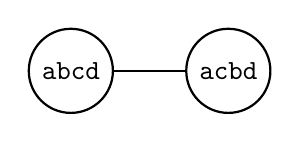
\begin{tikzpicture}
        [
        vertex/.style={circle,thick,draw,minimum size=2em},
        edge/.style={thick}
        ]
    \node[vertex] (1) at (0,0) {\lin{abcd}};
    \node[vertex] (2) at (2,0) {\lin{acbd}};
    \draw[edge] (1) -- (2);
    \end{tikzpicture}
    \caption{Swap graph $\sgraph{\lang{\poset{P}}}$ for $\poset{P}$ from Example~\ref{example:posetp}.}
    \label{figure:graphlp}
\end{figure}
\vspace{-15px}

We can exploit this property that a swap graph of poset language is connected to avoid exponential blow-up, by ``insulating'' each closed* connected component $\upsilon \subseteq \sgraph{\Upsilon}$ with a set $moat(\upsilon) = \set{\poset{L} \!\not\in\! \upsilon \mid \text{there is } \poset{L}' \!\in\! \upsilon \text{ such that } \poset{L}' \swap \poset{L}}$ that encloses it. We denote* by $moat(\Upsilon)$ the set $\bigcup_{\upsilon \in comp(\Upsilon)} moat(\upsilon)$, where $comp(\Upsilon)$ is the family of all closed connected components in $\Upsilon$.

\comment{(1) Is ``closed'' connected component an accepted term?\\(2) I replaced ``barrier'' with ``moat''.\\(3) I try $moat(\Upsilon)$ to reduce one quantifer. Is this actually better/clearer?}

An alternative way to encode $\Upsilon \supseteq \bigcup_{\poset{P} \in C} \lang{\poset{P}}$ is then
\[
\bigwedge_{\poset{L} \in moat(\Upsilon)} \bigwedge_{\poset{P} \in C} \poset{P} \not\lext \poset{L}
\]
This is polynomial in $\abs{\Upsilon}$ since $\abs{moat(\Upsilon)} \!\in\! \bigo{\abs{\Upsilon} \!\cdot\! \abs{\uni}}$ as the worst case is where every component is of size 1 and hence its moat contains all the posets which are one swap away from it.

\begin{proposition}
    Swap graph method is equivalent to naive method.
\end{proposition}
\begin{proof}
    Suppose the moat constraints hold. If the naive constraints do not hold, then there are some $\poset{L} \!\not\in\! \Upsilon$ and $\poset{P} \!\in\! C$ such that $\poset{P} \lext \poset{L}$. Per assumption, $\poset{L} \!\not\in\! moat(\Upsilon)$, but then $\sgraph{\lang{\poset{P}}}$ is not connected, a contradiction. The converse holds by definition, as $moat(\Upsilon) \subseteq \complmt{\Upsilon}$.
\end{proof}

\subsection{Some More Improvements}
% var better
We encode it as
\[
\bigwedge_{\poset{L} \in \Upsilon} \bigvee_{\poset{P} \in C} \bigwedge_{x,y \in \complmt{\leq[\poset{L}]}} \neg \mathtt{P}_{x,y}^{\poset{P}}
\]
by interpreting $\lext$ in its contrapositive form*.

% divide and conquer

% think, what's more?



%%%%%%%%%%%%%%%%%%%%%%%%%%%%%%%%%%%%%%%%%%%%%%%%%%%%
\bye{
\section{Problem Definition?or Poset covered Problem}


The poset covered problem is: given a set of linearizations $\Upsilon$, find a set of posets $\mathcal{C}$, called a covered, such that $\Upsilon = \bigcup_{P \in C} \mathcal{L}(P)$ and that $\abs{\mathcal{C}}$ is minimal.

\begin{theorem}
    insulating barrier method where?
\end{theorem}

\section{SAT Encoding Part}
We use the boolean logic of z3 SMT solver from MS research. Since poset is connected, by contraposition, we can first divide and conquer on connected components of the swap graph, by solving each component individually.

We then check with incrementing number of posets to find the minimal number of posets to covered each component. We first encode the axioms of posets; namely, reflexivity, antisymmetry, and transitivity. Next, we encode the extension constraint with contraposition from input linearizations to reduce the number of variables. Finally, we encode the non-extension constraint with negation of extension constraint on the insulating barrier.

\section{Exp Part}
NOTE: how do i put graph here?

\section{Conclusions}

\section{References}
NOTE: how to use list?

\section{Appendix}

\begin{theorem}
    Permutations and Nerode
\end{theorem}

\begin{theorem}
    (Corollary of Szpilrajn extension theorem) For a partial order $\leq$, $\leq = \bigcap_{< \in \mathcal{E}(\leq)} <$.
\end{theorem}

\begin{theorem}
    (Heath and Nema) If $x \incomp y$ for $\leq$ and there is $< \in \mathcal{E}(\leq)$ such that $x \covered y$ for $<$, then there is $<' \in \mathcal{E}(\leq)$ such that $y \covered x$ for $<'$.
\end{theorem}

\begin{theorem}
    Swap graphs are connected by Kendall tau paths
\end{theorem}

\begin{theorem}
    %(Szpilrajn Theorem) For a partial order $\poset{P}$, there exists a linear order $\mathcal{L}$ that extends $\poset{P}$; that is, $\leq_{\poset{P}} \subseteq \leq_{\mathcal{L}}$.
    \label{theorem:szpilrajn}
\end{theorem}

\begin{theorem}
    (Pruesse? and Ruskey) For a poset $\poset{P}$, the swap graph $\mathcal{G}(\poset{P})$ is connected. cite???
\end{theorem}

}

\end{document}
